
\documentclass{beamer}
\usepackage[utf8]{inputenc}

\usetheme{Madrid}
\usecolortheme{default}
\usepackage{amsmath,amssymb,amsfonts,amsthm}
\usepackage{txfonts}
\usepackage{tkz-euclide}
\usepackage{listings}
\usepackage{adjustbox}
\usepackage{array}
\usepackage{tabularx}
\usepackage{gvv}
\usepackage{lmodern}
\usepackage{circuitikz}
\usepackage{tikz}
\usepackage{graphicx}

\setbeamertemplate{page number in head/foot}[totalframenumber]

\usepackage{tcolorbox}
\tcbuselibrary{minted,breakable,xparse,skins}



\definecolor{bg}{gray}{0.95}
\DeclareTCBListing{mintedbox}{O{}m!O{}}{%
  breakable=true,
  listing engine=minted,
  listing only,
  minted language=#2,
  minted style=default,
  minted options={%
    linenos,
    gobble=0,
    breaklines=true,
    breakafter=,,
    fontsize=\small,
    numbersep=8pt,
    #1},
  boxsep=0pt,
  left skip=0pt,
  right skip=0pt,
  left=25pt,
  right=0pt,
  top=3pt,
  bottom=3pt,
  arc=5pt,
  leftrule=0pt,
  rightrule=0pt,
  bottomrule=2pt,
  toprule=2pt,
  colback=bg,
  colframe=orange!70,
  enhanced,
  overlay={%
    \begin{tcbclipinterior}
    \fill[orange!20!white] (frame.south west) rectangle ([xshift=20pt]frame.north west);
    \end{tcbclipinterior}},
  #3,
}
\lstset{
    language=C,
    basicstyle=\ttfamily\small,
    keywordstyle=\color{blue},
    stringstyle=\color{orange},
    commentstyle=\color{green!60!black},
    numbers=left,
    numberstyle=\tiny\color{gray},
    breaklines=true,
    showstringspaces=false,
}
\begin{document}

\title 
{4.12.2}
\date{September 14,2025}


\author 
{EE25BTECH11065-Yoshita J}






\frame{\titlepage}
\begin{frame}{Question}
For which value of $k$ will the following pair of linear equations have no solution?
\begin{align*}
    3x + y &= 1 \\
    (2k - 1)x + (k - 1)y &= 2k + 1
\end{align*}

\end{frame}


\begin{frame}{Theoretical Solution}
The given system of equations is
\begin{table}[H]    
  \centering
  \begin{tabular}{|c|c|}
\hline
\textbf{Name} & \textbf{Value} \\ \hline
$\vec{A}$ & $\myvec{2 & 1 \\0 & 3}$ \\ \hline
\end{tabular}

  \caption{Answers}
  \label{Answers}
\end{table}
In matrix form:
\begin{align}
\myvec{3 & 1 \\ 2k-1 & k-1}\myvec{x \\ y} = \myvec{1 \\ 2k+1}
\end{align}

Now, form the augmented matrix:
\begin{align}
\augvec{2}{1}{3 & 1 &  1 \\ 2k-1 & k-1 & 2k+1}
\end{align}

\end{frame}

\begin{frame}{Theoretical Solution}
Perform row reduction:
\begin{align}
R_1 \to \tfrac{1}{3}R_1 
&\quad\Rightarrow\quad
\augvec{2}{1}{1 & \tfrac{1}{3} & \tfrac{1}{3} \\[6pt]
2k-1 & k-1 & 2k+1} \\[10pt]
%
R_2 \to R_2-(2k-1)R_1
&\quad\Rightarrow\quad
\augvec{2}{1}{1 & \tfrac{1}{3} & \tfrac{1}{3} \\[6pt]
0 & \tfrac{k-2}{3} & \tfrac{4k+4}{3}} \\[10pt]
%
R_2 \to \tfrac{3}{k-2}R_2
&\quad\Rightarrow\quad
\augvec{2}{1}{1 & \tfrac{1}{3} & \tfrac{1}{3} \\[6pt]
0 & 1 & \tfrac{4k+4}{k-2}} \\[10pt]
%
R_1 \to R_1-\tfrac{1}{3}R_2
&\quad\Rightarrow\quad
\augvec{2}{1}{1 & 0 & \tfrac{1}{3}-\tfrac{1}{3}\cdot\tfrac{4k+4}{k-2} \\[6pt]
0 & 1 & \tfrac{4k+4}{k-2}}
\end{align}
\end{frame}

\begin{frame}{Theoretical Solution}
For inconsistency, we need:
\begin{align}
k-2 = 0 \quad \text{and} \quad 4k+4 \neq 0
\end{align}
So,
\begin{align}
k = 2, \quad 4(2)+4 = 12 \neq 0
\end{align}

\begin{align*}
\boxed{k = 2}
\end{align*}
\end{frame}

\begin{frame}[fragile]
    \frametitle{C Code}

    \begin{lstlisting}
#include<stdio.h>
double solve_for_k(void) {
    double a1 = 3.0;
    double b1 = 1.0;
    double c1 = 1.0;
    double a2_k_coeff = 2.0;
    double a2_const = -1.0;
    double b2_k_coeff = 1.0;
    double b2_const = -1.0;
    double c2_k_coeff = 2.0;
    double c2_const = 1.0;
    double k_coeff_det = a1 * b2_k_coeff - b1 * a2_k_coeff;
    double const_det = a1 * b2_const - b1 * a2_const;
    double k = -const_det / k_coeff_det;

    return k;
}

    \end{lstlisting}
\end{frame}


\begin{frame}[fragile]
    \frametitle{Python Code}
    \begin{lstlisting}
import numpy as np
import matplotlib.pyplot as plt

k_value = 2.0
print(f"The value of k for which there is no solution is:")
print(f"  k = {k_value:.2f}")

x = np.linspace(-5, 5, 100)

y1 = 1 - 3 * x

y2 = (2 * k_value + 1 - (2 * k_value - 1) * x) / (k_value - 1)

plt.figure(figsize=(8, 6))
plt.plot(x, y1, label=r'$3x + y = 1$')
plt.plot(x, y2, label=f'${{{(2*k_value-1):.0f}}}x + {{{(k_value-1):.0f}}}y = {{{(2*k_value+1):.0f}}}$ (for k={k_value:.0f})', linestyle='--')



    \end{lstlisting}
\end{frame}

\begin{frame}[fragile]
    \frametitle{Python Code}
    \begin{lstlisting}
plt.xlabel('X-axis')
plt.ylabel('Y-axis')
plt.title(f'Lines for k = {k_value:.2f} (No Solution)', fontsize=14)
plt.axhline(0, color='black',linewidth=0.5)
plt.axvline(0, color='black',linewidth=0.5)
plt.grid(color = 'gray', linestyle = '--', linewidth = 0.5)
plt.legend()
plt.show()
   
    \end{lstlisting}
\end{frame}


\begin{frame}{Plot}
    \centering
    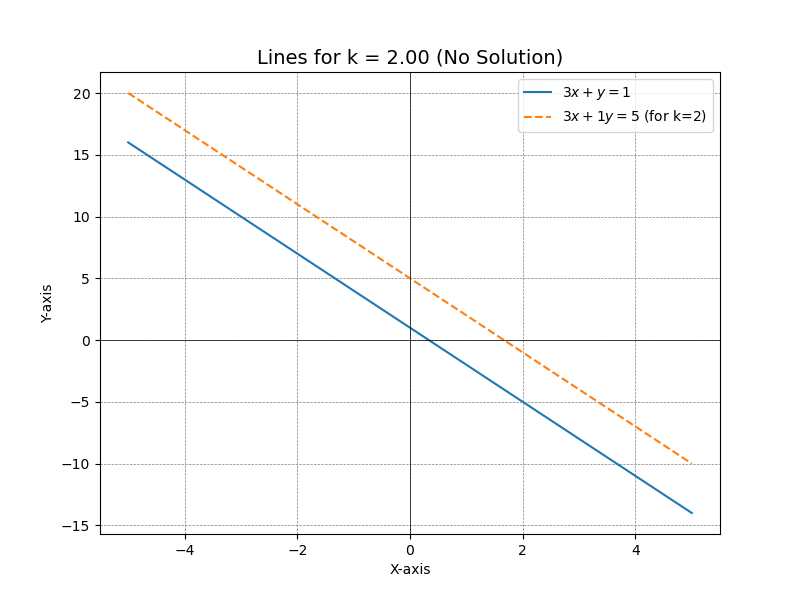
\includegraphics[width=\columnwidth, height=0.9\textheight, keepaspectratio]{figs/fig5.png}     
\end{frame}


\end{document}
